%%%%%%%%%%%%%%%%%%%%%%%%%%%%%%%%%%%%%%%%%%%%%%%%%%%%%%%%%%%%%%%%%%%%%%%%%%%%%%%%%%%%%%%%%%%%%%%%%%%%%%
%%%%%%%%%%%%%% Template de Artigo Adaptado para Trabalho de Conclusão de Curso - SI Contagem - PUCMINAS %%%%%%%%%%%%%%%%%%%%%%%%
%% codificação UTF-8 - Abntex - Latex -  							     %%
%% Autor da primeira versão:    Fábio Leandro Rodrigues Cordeiro  (fabioleandro@pucminas.br)                            %% 
%% Co-autor da primeira versão: Prof. João Paulo Domingos Silva, Harison da Silva e Anderson Carvalho.                   %%
%% Revisores normas NBR (Padrão PUC Minas) da primeira versão: Helenice Rego Cunha e Prof. Theldo Cruz.                   %%
%% Versão: 1.1     18 de dezembro de 2015 
%% Revisora normas NBR (Padrão PUC Minas) da terceira versão: Profa. Amália Vasconcelos.                   %%
%% Versão: 3.0     02 de fevereiro de 2026 
%%%%%%%%%%%%%%%%%%%%%%%%%%%%%%%%%%%%%%%%%%%%%%%%%%%%%%%%%%%%%%%%%%%%%%%%%%%%%%%%%%%%%%%%%%%%%%%%%%%%%%

%\textcolor{red}{\textbf{Importante:}} mantenha atualizada a versão do TeX Live. No Overleaf, escolha o "motor" de compilação no menu \texttt{File >\allowbreak\ Settings >\allowbreak\ Compiler >\allowbreak\ TeX Live version >\allowbreak\ selecione a mais atual}. Ex.: 2025.

\documentclass[a4paper,12pt]{article}
\usepackage{times}
\usepackage{abakos}  %pacote com padrão da Abakos baseado no padrão da PUC
\usepackage[hidelinks]{hyperref}
\providecommand{\htmladdnormallink}[2]{\href{#2}{#1}}

\makeatletter
% Trecho adicionado, pois na ABNT NBR 6023:2002, URLs em referências ficavam entre <...>. A partir da 6023:2018 não ficam mais.
\AddToHook{env/thebibliography/begin}{%
  \def\UrlLeft{}%
  \def\UrlRight{}%
  \urlstyle{same}%
}
\makeatother

%%%%%%%%%%%%%%%%%%%%%%%%%%%
%Capa da revista
%%%%%%%%%%%%%%%%%%%%%%%%%%

%\setcounter{page}{80} %iniciar contador de pagina de valor especificado
\newcommand{\monog}{A Implementação de um Mapa Interativo Sobre as Empresas de TI do Município de Contagem}
%\newcommand{\monogES}{Article template Institute of Mathematical Sciences and Informatics}
\newcommand{\tipo}{Artigo}  % Especificar a seção tipo do trabalho: Artigo, Resumo, Tese, Dociê etc
%\newcommand{\origem}{Brasil}
%\newcommand{\editorial}{Belo Horizonte, p. 01-11, nov. 2024}  % p. xx-xx – páginas inicial-final do artigo
\newcommand{\editorial}{}  
\newcommand{\lcc}{{\scriptsize Licença Creative Commons Attribution-NonCommercial-NoDerivatives 4.0 International License}}

%%%%%%%%%%%%%%%%%INFORMAÇÕES SOBRE AUTOR PRINCIPAL %%%%%%%%%%%%%%%%%%%%%%%%%%%%%%%
\newcommand{\AutorA}{Matheus Canuto}
\newcommand{\funcaoA}{}
\newcommand{\emailA}{\href{mailto:[E-MAIL]@sga.pucminas.br}{[E-MAIL]@sga.pucminas.br}}
\newcommand{\cursA}{Aluno do Programa de Graduação em Sistemas de Informação}

\newcommand{\AutorB}{Paulo Henrique Rodrigues}
\newcommand{\funcaoB}{}
\newcommand{\emailB}{\href{mailto:496762@pucminas.edu.br}{496762@pucminas.edu.br}}
\newcommand{\cursB}{Professor do Programa de Graduação em Sistemas de Informação}

% --- Avaliadores heurísticos (NÃO são coautores; nomes também na Metodologia) ---
% Orientador (também avaliador): Paulo Henrique Rodrigues | 496762@pucminas.edu.br
% Colega avaliador 1 (desenvolvedor): [NOME COMPLETO COLEGA 1] | [E-MAIL COLEGA 1] | [MATRÍCULA COLEGA 1]
% Colega avaliador 2 (desenvolvedor): [NOME COMPLETO COLEGA 2] | [E-MAIL COLEGA 2] | [MATRÍCULA COLEGA 2]
%
% Definir macros para o nome da Instituição, da Faculdade, etc.
\newcommand{\univ}{Pontifícia Universidade Católica de Minas Gerais}

\newcommand{\keyword}[1]{\textsf{#1}}

%Para as URLS não ultrapassarem a margem
\usepackage{url}
\makeatletter
\g@addto@macro{\UrlBreaks}{\UrlOrds}
\makeatother

\usepackage{adjustbox} % reduzir tamanho figuras
\usepackage{float} % posição [H] para fixar figura no ponto do texto

\usetikzlibrary{arrows,arrows.meta,shapes,positioning,shadows,trees}

\tikzset{
  basic/.style  = {draw, text width=3cm, drop shadow, font=\sffamily, rectangle},
  root/.style   = {basic, rounded corners=2pt, thin, align=center,
                   fill=blue!30},
  level 2/.style = {basic, rounded corners=6pt, thin,align=center, fill=green!30,
                   text width=8em},
  level 3/.style = {basic, thin, align=left, fill=pink!60, text width=6.5em}
}

\begin{document}
% %%%%%%%%%%%%%%%%%%%%%%%%%%%%%%%%%%
% %% Página de título
% %%%%%%%%%%%%%%%%%%%%%%%%%%%%%%%%%%

\begin{center}
\includegraphics[scale=0.25]{figuras/brasao} \\
PONTIFÍCIA UNIVERSIDADE CATÓLICA DE MINAS GERAIS \\
Instituto de Ciências Exatas e de Informática

% \vspace{1.0cm}

\end{center}

 \vspace{0cm} {
 \singlespacing \Large{\monog \symbolfootnote[1]{Artigo apresentado ao Instituto de Ciências Exatas e Informática da Pontifícia Universidade Católica de \linebreak Minas Gerais, campus Contagem, como pré-requisito parcial para obtenção do título de Bacharel em Sistemas de Informação.} \\ }
 % \normalsize{\monogES}
 }

\vspace{1.0cm}

\begin{flushright}
\singlespacing 
\normalsize{\AutorA \footnote{\funcaoA \cursA \,-- \emailA . }} \\
\normalsize{\AutorB \footnote{\funcaoB \cursB \,-- \emailB . }} \\
%\normalsize{\AutorC \footnote{\funcaoC \cursC \,-- \emailC . }} \\
%\normalsize{\AutorD \footnote{\funcaD \cursD \,-- \emailD . }} \\
\end{flushright}
\thispagestyle{empty}

\vspace{1.0cm}

\begin{abstract}
\noindent
Os dados públicos sobre empresas estão em arquivos extensos, espalhados por mais de uma instituição, o que dificulta a consulta por quem não tem familiaridade com tabelas. Embora Contagem (MG) cumpra a legislação de acesso à informação, não há um sistema de consulta de fácil compreensão sobre suas empresas de Tecnologia da Informação (TI). Aproximar esses dados de cidadãos, profissionais e empresários justifica o estudo. O objetivo é desenvolver uma aplicação web interativa que caracterize e apresente essas empresas a partir da integração de dados abertos. Foram integrados em um banco MySQL a base de CNPJ da Receita Federal, a CNAE e o CNEFE do IBGE, e a aplicação, feita com SvelteKit e Leaflet, reúne mapa, indicadores, tabela e filtros, com usabilidade avaliada pelo System Usability Scale (SUS). A base reuniu 781 estabelecimentos ativos na fotografia de 13/10/2026 da Receita Federal, dos quais 86,6\% são microempresas e 82,1\% receberam coordenada pelo CEP. Conclui-se que é possível integrar essas bases em uma consulta única, mas a coordenada é aproximada e a ligação por endereço é a etapa mais frágil.
\\\textbf{\keyword{Palavras-chave:}} dados abertos; empresas de tecnologia da informação; visualização de dados; geocodificação; Contagem.
\end{abstract}

%%%%%%%%%%%%%%%%%%%%%%%%%%%%%%%%%%%%%%%%%%%%%%%%%%%%%%%%%
% Resumo em inglês desativado para cumprir o limite de 15 páginas do regulamento (reativar removendo \iffalse e \fi).
\iffalse
\selectlanguage{english}
\begin{abstract}
\noindent
Public data on companies are published in large files spread across more than one institution, which makes them hard to query for people unfamiliar with spreadsheets. Although Contagem (MG, Brazil) complies with access-to-information legislation, there is no easy-to-understand query system about its Information Technology (IT) companies. Bringing these data closer to citizens, professionals and entrepreneurs justifies the study. The goal is to develop an interactive web application that characterizes and presents these companies from the integration of open data. The Federal Revenue company registry (CNPJ), the CNAE activity classification and the CNEFE address registry from IBGE were integrated into a MySQL database, and the application, built with SvelteKit and Leaflet, combines a map, indicators, a table and filters, with usability assessed by the System Usability Scale (SUS). The database gathered 781 active establishments from the Federal Revenue snapshot of 13 October 2026, 86.6\% of which are microenterprises and 82.1\% received coordinates by postal code. It is concluded that these databases can be integrated into a single query tool, but the coordinates are approximate and address matching is the most fragile step.
\\\textbf{\keyword{Keywords:}} open data; information technology companies; data visualization; geocoding; Contagem.
\end{abstract}
\fi

\selectlanguage{brazilian}
 \onehalfspace  % espaçamento 1.5 entre linhas
 \setlength{\parindent}{1.25cm}

%%%%%%%%%%%%%%%%%%%%%%%%%%%%%%%%%%%%%%%%%%%%%%%%%
%% INÍCIO DO TEXTO
%%%%%%%%%%%%%%%%%%%%%%%%%%%%%%%%%%%%%%%%%%%%%%%%%

\section{Introdução}

No Brasil, o acesso a informações públicas é um direito garantido pela Lei de Acesso à Informação (LAI), Lei nº 12.527, de 18 de novembro de 2011 \cite{brasil2011}.
A LAI obriga os órgãos públicos a divulgar, por iniciativa própria, informações de interesse coletivo em meios eletrônicos e em formatos abertos, e a responder aos pedidos de informação apresentados por qualquer pessoa.
Para além da LAI, outras legislações, como a Lei da Transparência, Lei Complementar nº 131, de 27 de maio de 2009 \cite{brasil2009}, garantem o acesso da população a informações importantes da esfera pública, ao exigir a divulgação, em tempo real, da execução orçamentária e financeira da União, dos estados e dos municípios.

O uso de dados para compreender a dinâmica econômica de um município pode contribuir para a identificação de características relacionadas à distribuição das atividades econômicas, à ocupação territorial e ao desenvolvimento de determinados setores.
Nesse contexto, dados produzidos e mantidos por órgãos públicos podem ser utilizados não apenas para fins administrativos, mas também para produzir informações que auxiliem cidadãos, empresas, pesquisadores e gestores na compreensão do ambiente econômico local.

Contagem integra a Região Metropolitana de Belo Horizonte e tinha 621.863 habitantes no Censo Demográfico de 2022, em uma área de cerca de 195 km\textsuperscript{2} \cite{ibge2026}.
Em 2023, o Produto Interno Bruto do município foi de R\$ 45,1 bilhões, o quarto maior de Minas Gerais \cite{ibge2026}.
Embora a cidade seja conhecida pela indústria, a maior parte da riqueza gerada vem do setor terciário, o de serviços, do qual fazem parte as empresas de Tecnologia da Informação: em 2021, os serviços responderam por 59,1\% do valor adicionado bruto municipal, e a indústria, por 30,8\% \cite{ibge2026}.

Contagem está adequada à legislação de acesso à informação.
Em 2025, o município recebeu pela segunda vez consecutiva o Selo Ouro do Programa Nacional de Transparência Pública, com índice de 85,64\% no Radar da Transparência, por atender a todos os itens considerados essenciais na avaliação \cite{contagem2025}.
A própria prefeitura declara manter um banco de dados das atividades econômicas do município, com os registros classificados pela Classificação Nacional de Atividades Econômicas (CNAE) e com geolocalização \cite{contagem2026}.
Esses dados, porém, não são oferecidos ao público em um sistema de consulta de fácil compreensão.

O cumprimento da legislação de acesso à informação nem sempre é garantia de facilidade de acesso e leitura dos dados.
Segundo \citeonline{ansari2022}, o aumento da quantidade de dados governamentais publicados não resultou, por si só, em maior uso dessas informações pela sociedade.
Os mesmos autores apontam a visualização de dados como um caminho para reduzir essa distância entre a publicação e o uso.

Diante desse cenário, este trabalho busca responder à seguinte questão de pesquisa: é possível combinar os dados disponibilizados pela legislação para criar um sistema interativo que facilite a visualização dos dados referentes às empresas de TI do município de Contagem?

O objetivo geral deste trabalho é desenvolver uma aplicação web interativa que permita caracterizar e visualizar as empresas do setor de Tecnologia da Informação do município de Contagem a partir da integração de dados abertos.
A aplicação reunirá indicadores, gráficos, mapas, tabelas e mecanismos de filtragem, ajustados à estrutura e à qualidade das fontes utilizadas.

Como objetivos específicos, pretende-se:

\begin{itemize}
    \item coletar e tratar dados abertos sobre os estabelecimentos de Tecnologia da Informação de Contagem, integrando atividade econômica, porte e localização em uma base única;
    \item projetar uma aplicação web para a consulta desses dados, com levantamento de requisitos, diagrama de casos de uso e esquema do banco de dados;
    \item implementar essa aplicação, de modo que o usuário possa consultar, filtrar e interpretar as informações por meio de mapa, gráficos e tabelas;
    \item testar a aplicação, conferindo a localização atribuída aos estabelecimentos e avaliando a usabilidade da interface por meio da System Usability Scale (SUS).
\end{itemize}

Todos os dados utilizados no sistema foram coletados em fontes públicas oficiais, ou seja, já estão publicados.
Ainda assim, foi observada a Lei Geral de Proteção de Dados Pessoais (LGPD), Lei nº 13.709, de 14 de agosto de 2018 \cite{brasil2018}.
Dados pessoais, como nome e CPF de sócios, não foram divulgados.

A relevância deste estudo justifica-se pela necessidade de aproximar dados públicos, hoje muitas vezes dispersos e difíceis de consultar devido à sua apresentação, de públicos que podem utilizá-los na prática, como os cidadãos, que poderão conhecer melhor as empresas de tecnologia existentes no município; os profissionais, que poderão identificar organizações relacionadas às suas áreas de interesse; os empresários, que poderão conhecer empresas do mesmo setor e identificar possíveis fornecedores ou parceiros; e os empreendedores, que poderão explorar características da distribuição das atividades econômicas no município.

Sob a perspectiva acadêmica, o trabalho contribui para a área de Sistemas de Informação ao integrar dados abertos, análise descritiva e visualização interativa em um recorte municipal concreto, alinhado a estudos que relacionam localização e setor de tecnologia em contextos urbanos, como o de \citeonline{zenka2021}.
A escolha do tema pauta-se na formação em Sistemas de Informação e no interesse por soluções que transformem bases públicas em instrumentos de consulta e interpretação para usuários não especializados.

Este trabalho está estruturado em seis seções.
Após esta introdução, a Seção 2 apresenta o referencial teórico, e a Seção 3 os trabalhos relacionados.
A Seção 4 descreve a metodologia empregada, incluindo a coleta e a integração das bases de dados abertos e o projeto da aplicação web.
A Seção 5 apresenta o software desenvolvido e os testes da aplicação.
Por fim, a Seção 6 apresenta as conclusões do trabalho, suas limitações e as possibilidades de continuidade da pesquisa.

\section{Referencial Teórico}

Esta seção apresenta os conceitos que sustentam o trabalho.

\subsection{Dados abertos governamentais}

Dados abertos governamentais são informações produzidas ou mantidas pelo poder público e disponibilizadas para que outras pessoas possam usá-las de novo.
O objetivo costuma ser aumentar a transparência e permitir que esses dados sejam reaproveitados.
\citeonline{molodtsov2024} estudaram a usabilidade de portais de dados abertos em 33 países.
O quadro que eles aplicam não olha só se o arquivo está disponível para \textit{download}.
Também entra se a pessoa consegue explorar o dado e entendê-lo, mesmo sem prática com planilha.
\citeonline{ansari2022}, ao revisar pesquisas sobre visualização de dados governamentais, observam um ponto parecido: publicar o arquivo não faz, por si só, com que o dado seja usado.
Muita gente não consegue ler o formato, cruzar bases diferentes e interpretar a tabela.
Uma aplicação que junta as bases e mostra mapa, gráfico e filtro pode tornar essa consulta mais simples.
Esse é o caminho deste trabalho: caracterizar as empresas de TI de Contagem a partir de bases abertas nacionais, e não a partir de um arquivo municipal já pronto.

\subsection{System Usability Scale (SUS)}

Usabilidade, neste trabalho, é a facilidade de usar a interface.
A pessoa encontra a informação, entende o que está vendo e consegue filtrar sem se perder.
A System Usability Scale (SUS), proposta por \citeonline{brooke1996}, é um questionário de dez itens em escala Likert de cinco pontos, com afirmações alternadas entre positivas e negativas.
Após o uso do sistema, cada participante responde aos itens; a pontuação individual é convertida para uma escala de 0 a 100.
Essa medida única resume a percepção global de usabilidade e permite comparar o resultado com faixas de interpretação usadas na literatura.
Este trabalho aplica o SUS à aplicação desenvolvida, após os participantes percorrerem o mapa, os filtros, os indicadores e a tabela.

\subsection{Classificação Nacional de Atividades Econômicas (CNAE)}

A identificação de um setor em cadastros públicos depende de uma classificação padronizada das atividades.
No Brasil, a Classificação Nacional de Atividades Econômicas (CNAE), mantida pelo IBGE, é o instrumento usado pelo sistema estatístico e pelos órgãos que registram empresas \cite{ibge2020}.
A CNAE organiza as atividades em níveis, da seção até a subclasse.
No CNPJ, cada estabelecimento tem um código de atividade principal.

Neste trabalho, empresa de TI é o estabelecimento cuja atividade principal está na divisão 62, de serviços de tecnologia da informação, na versão CNAE-Subclasses 2.3.
Os códigos são 6201-5/01 (desenvolvimento de programas sob encomenda), 6201-5/02 (web design), 6202-3/00 (programas customizáveis), 6203-1/00 (programas não customizáveis), 6204-0/00 (consultoria em tecnologia da informação) e 6209-1/00 (suporte técnico e outros serviços em TI).
Não entram a divisão 63 (hospedagem, tratamento de dados e portais), o comércio e a fabricação de equipamentos, o conserto de computador nem o curso de informática.
A regra usa só a atividade principal, para a lista não crescer com códigos secundários de empresas de outro ramo.

\section{Trabalhos Relacionados}

\citeonline{barretojunior2021} desenvolveram o Buskaki Empresas, uma aplicação web para consultar empresas de Curitiba por campos além do CNPJ, como a razão social e o nome fantasia.
A ferramenta usa os dados abertos da Receita Federal, foi construída com Ruby on Rails, PostgreSQL e PostGIS e geocodifica os endereços por um serviço externo, que, segundo os autores, chegou a deslocar o ponto em até 2 km em alguns casos.
Como resultado, a aplicação permite buscar a empresa pelo nome ou pelo CNPJ, listar as empresas por bairro e por rua e ver cada uma em um mapa dinâmico.
O foco do Buskaki é encontrar uma empresa específica, e não caracterizar um setor; a consulta exige cadastro, e os testes com usuários ficaram como trabalho futuro.

\citeonline{silva2024} apresentaram a base de CNPJ da Receita Federal como fonte para estudos espaciais na Geografia urbana, econômica e regional.
As autoras integraram as tabelas da base pelo CNPJ básico, selecionaram municípios e códigos da CNAE, padronizaram os campos de endereço e geocodificaram os registros em \textit{software} de geoprocessamento.
Em Presidente Prudente, 51.484 dos 52.876 CNPJs ativos selecionados receberam coordenada, e a perda em outras cidades não passou de 5\%; o artigo também aponta limitações da base, como registros duplicados e muitos CNPJs em um mesmo endereço residencial.
O estudo é metodológico e não entrega uma aplicação: os mapas são figuras estáticas produzidas pelas pesquisadoras, sem registro da precisão do ponto de cada estabelecimento.

O Mapa de Empresas é uma ferramenta do Governo Federal que publica mensalmente informações sobre o registro de empresas no país, a partir da base do CNPJ \cite{brasil2026}.
O painel mostra empresas abertas, fechadas e ativas, permite filtrar por atividade econômica, natureza jurídica, porte e município e exporta gráficos, mapas e tabelas com os filtros aplicados.
O manual recomenda registrar a data da consulta e os filtros usados, porque os números podem ser revistos em cargas posteriores, cuidado que este trabalho adota com a data da fotografia das bases.
Os resultados são agregados: é possível saber quantas empresas de uma atividade existem em Contagem, mas o painel não lista nem localiza cada estabelecimento dentro do município.

Os três trabalhos partem da base de CNPJ, como este, e os dois acadêmicos enfrentam o mesmo problema: o endereço não traz coordenada, e a geocodificação perde ou desloca parte dos registros.
Nenhum deles reúne, em uma aplicação aberta e sem cadastro, a caracterização de um setor dentro de um município, a localização de cada estabelecimento com a indicação da precisão da coordenada e uma avaliação de usabilidade da interface.
Este trabalho busca preencher essa lacuna para as empresas de TI de Contagem, ao combinar a base de CNPJ, a coordenada do CNEFE e um \textit{dashboard} em que indicadores, mapa e tabela respondem aos mesmos filtros.

\section{Metodologia}

Este trabalho tem como objetivo desenvolver uma aplicação web interativa que caracterize e apresente as empresas de Tecnologia da Informação do município de Contagem a partir da integração de dados abertos.
Bases públicas sobre estabelecimentos, atividades econômicas e endereços foram coletadas, tratadas e combinadas em um banco de dados único, que alimenta a aplicação com mapa, indicadores, tabelas e filtros.
A usabilidade da interface foi avaliada com a System Usability Scale (SUS).

Quanto à natureza, a pesquisa é aplicada, pois resulta em uma aplicação web.
Quanto aos objetivos, é descritiva, por caracterizar os estabelecimentos de TI de um município \cite{gil2008}.
Quanto aos procedimentos, combina pesquisa documental em bases públicas com o desenvolvimento de software.
A abordagem é quantitativa na descrição dos dados e na pontuação do SUS.

O trabalho foi realizado nas seguintes etapas:

\begin{enumerate}
    \item coleta e tratamento dos dados (CNPJ, CNAE, CNEFE e malhas do IBGE, integrados em MySQL);
    \item projeto da solução (requisitos, casos de uso e esquema do banco);
    \item implementação da solução (programa de carga e aplicação web);
    \item testes (conferência da localização, comparação com o CEMPRE e avaliação SUS).
\end{enumerate}

Na primeira etapa ocorreu a coleta e o tratamento dos dados.
Foi feita a pesquisa das fontes oficiais e o \textit{download} dos arquivos publicados.
A lista de estabelecimentos veio da base pública de CNPJ da Receita Federal do Brasil, com identificação, situação cadastral, porte e endereço declarado; o arquivo de sócios não foi utilizado.
Os dados considerados foram os da divisão 62 da CNAE-Subclasses 2.3, conforme o recorte definido no referencial teórico.
As coordenadas vieram do Cadastro Nacional de Endereços para Fins Estatísticos (CNEFE) do Censo Demográfico 2022, do IBGE.
As malhas territoriais do IBGE forneceram o contorno do município, e tabelas do Cadastro Central de Empresas (CEMPRE), via SIDRA, serviram para conferência dos totais.
O objeto de análise ficou restrito a Contagem (código IBGE 3118601), com estabelecimentos em situação cadastral ativa na fotografia das bases, unidade igual ao estabelecimento do CNPJ (matriz e filial contam separadas quando ambas estão no município e na atividade escolhida).

Ainda na primeira etapa, o tratamento foi feito em ambiente local, por um programa em Python.
Em linhas gerais, o script faz requisições às fontes públicas, baixa os arquivos, lê os CSV, aplica os filtros do recorte e transforma o resultado em SQL para carga no MySQL.
Primeiro, o programa obteve e leu os arquivos.
Em seguida, filtrou Contagem e as subclasses da divisão 62, antes de qualquer junção.
Depois, integrou as bases por chaves explícitas: o CNPJ básico uniu o estabelecimento aos dados da empresa, como razão social, porte e capital social; o código de atividade padronizou a subclasse; e o código IBGE 3118601 isolou o município.
O endereço passou por padronização (CEP com oito dígitos, texto em maiúsculas sem acento e expansão de abreviações de logradouro) e foi ligado ao CNEFE por níveis sucessivos: endereço completo, só CEP ou sem coordenada.
O resultado foi gravado em um banco MySQL, com a data da fotografia das bases.
A aplicação consulta esse banco, e não os arquivos nacionais nem os sites da Receita e do IBGE.

Na segunda etapa ocorreu o projeto da solução.
Foram levantados os requisitos funcionais e não funcionais, elaborados o diagrama de casos de uso e o esquema do banco de dados.
Os requisitos funcionais e não funcionais definidos constam nas Tabelas \ref{tab:rf} e \ref{tab:rnf}.

\begin{table}[htbp]
    \centering
    \caption{Requisitos funcionais da aplicação}
    \label{tab:rf}
    \begin{tabular}{|c|p{11.5cm}|}
        \hline
        \textbf{Código} & \textbf{Descrição} \\
        \hline
        RF01 & Exibir indicadores gerais, como o total de estabelecimentos e a distribuição por subclasse e por porte. \\
        \hline
        RF02 & Filtrar por subclasse, porte, condição de MEI e disponibilidade de coordenada. \\
        \hline
        RF03 & Exibir os estabelecimentos em um mapa de pontos. \\
        \hline
        RF04 & Listar os estabelecimentos em uma tabela com busca. \\
        \hline
        RF05 & Informar a data da fotografia das bases e se há coordenada. \\
        \hline
    \end{tabular}
    \\\textbf{\footnotesize Fonte: Elaborado pelo autor.}
\end{table}

\begin{table}[htbp]
    \centering
    \caption{Requisitos não funcionais da aplicação}
    \label{tab:rnf}
    \begin{tabular}{|c|p{11.5cm}|}
        \hline
        \textbf{Código} & \textbf{Descrição} \\
        \hline
        RNF01 & Acesso pelo navegador, sem cadastro de usuário. \\
        \hline
        RNF02 & Não exibir CPF, quadro de sócios, telefone ou e-mail. \\
        \hline
        RNF03 & Indicadores, mapa e tabela respondendo aos mesmos filtros. \\
        \hline
        RNF04 & Consultas feitas no banco da aplicação, sem depender de serviço externo além do mapa de fundo. \\
        \hline
    \end{tabular}
    \\\textbf{\footnotesize Fonte: Elaborado pelo autor.}
\end{table}

A Figura \ref{fig:casos-de-uso} apresenta o diagrama de casos de uso.
O visitante consulta indicadores, aplica filtros, explora o mapa e a tabela e vê a data da fotografia.
O administrador, papel exercido pelo autor, carrega uma nova fotografia das bases.

\begin{figure}[H]
    \centering
    \caption{Diagrama de casos de uso da aplicação}
    \label{fig:casos-de-uso}
    \vspace{-0.2cm}
    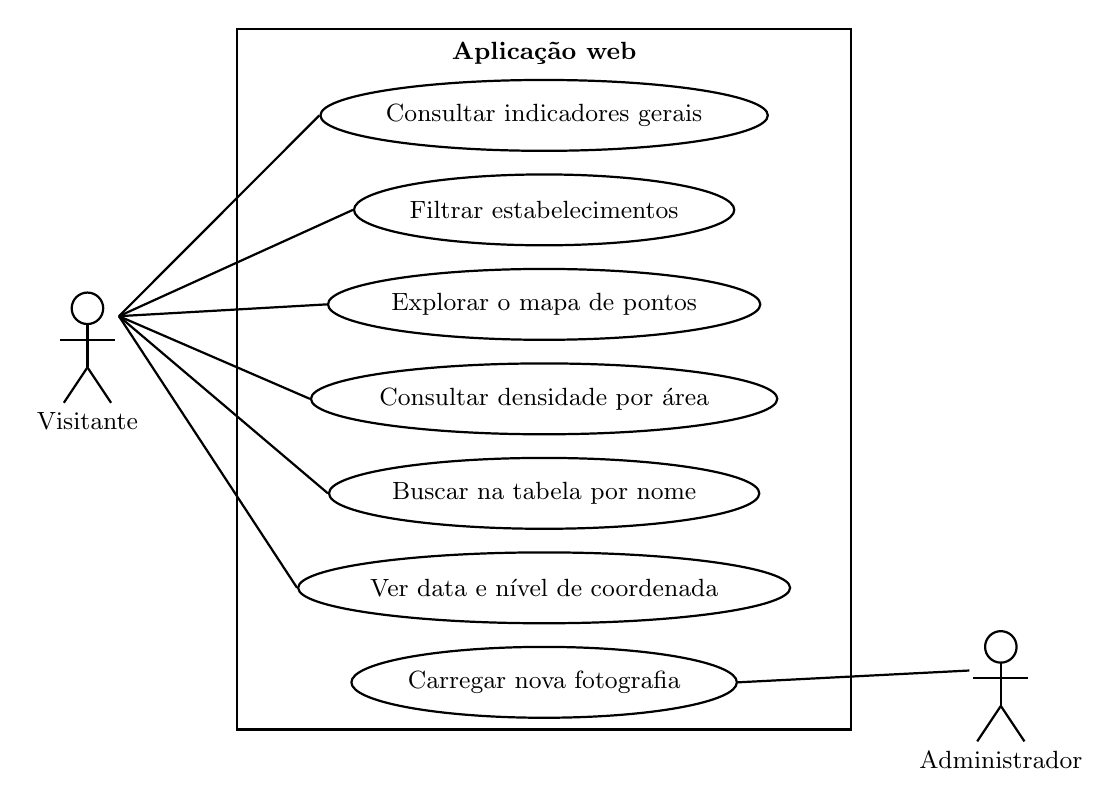
\begin{tikzpicture}[
        caso/.style={
            draw=black,
            thick,
            ellipse,
            font=\small,
            inner sep=0pt,
            minimum height=0.9cm
        },
        assoc/.style={thick},
        ator/.pic={
            \draw[thick] (0,1.05) circle (0.2);
            \draw[thick] (0,0.85) -- (0,0.3);
            \draw[thick] (-0.35,0.65) -- (0.35,0.65);
            \draw[thick] (0,0.3) -- (-0.3,-0.15);
            \draw[thick] (0,0.3) -- (0.3,-0.15);
        }
    ]
        \draw[thick] (-3.9,4.0) rectangle (3.9,-4.9);
        \node[font=\small\bfseries, anchor=north] at (0,3.95) {Aplicação web};

        \node[caso] (uc1) at (0,2.9) {Consultar indicadores gerais};
        \node[caso] (uc2) at (0,1.7) {Filtrar estabelecimentos};
        \node[caso] (uc3) at (0,0.5) {Explorar o mapa de pontos};
        \node[caso] (uc4) at (0,-0.7) {Consultar densidade por área};
        \node[caso] (uc5) at (0,-1.9) {Buscar na tabela por nome};
        \node[caso] (uc6) at (0,-3.1) {Ver data e nível de coordenada};
        \node[caso] (uc7) at (0,-4.3) {Carregar nova fotografia};

        \pic at (-5.8,-0.6) {ator};
        \node[font=\small, below] at (-5.8,-0.75) {Visitante};
        \coordinate (v) at (-5.4,0.35);
        \foreach \uc in {uc1,uc2,uc3,uc4,uc5,uc6} {
            \draw[assoc] (v) -- (\uc.west);
        }

        \pic at (5.8,-4.9) {ator};
        \node[font=\small, below] at (5.8,-5.05) {Administrador};
        \draw[assoc] (5.4,-4.15) -- (uc7.east);
    \end{tikzpicture}
    \vspace{-0.2cm}
    \\\textbf{\footnotesize Fonte: Elaborado pelo autor.}
\end{figure}


A Figura \ref{fig:esquema-banco} apresenta o esquema do banco MySQL.
Cada estabelecimento se liga à empresa pelo CNPJ básico, à atividade pela subclasse e à carga em que foi gravado.
A localização guarda a coordenada e o nível de junção com o CNEFE.
A carga registra a data da fotografia e as versões das bases.

\begin{figure}[H]
    \centering
    \caption{Esquema do banco de dados da aplicação}
    \label{fig:esquema-banco}
    \vspace{-0.2cm}
    \renewcommand{\arraystretch}{1.1}
    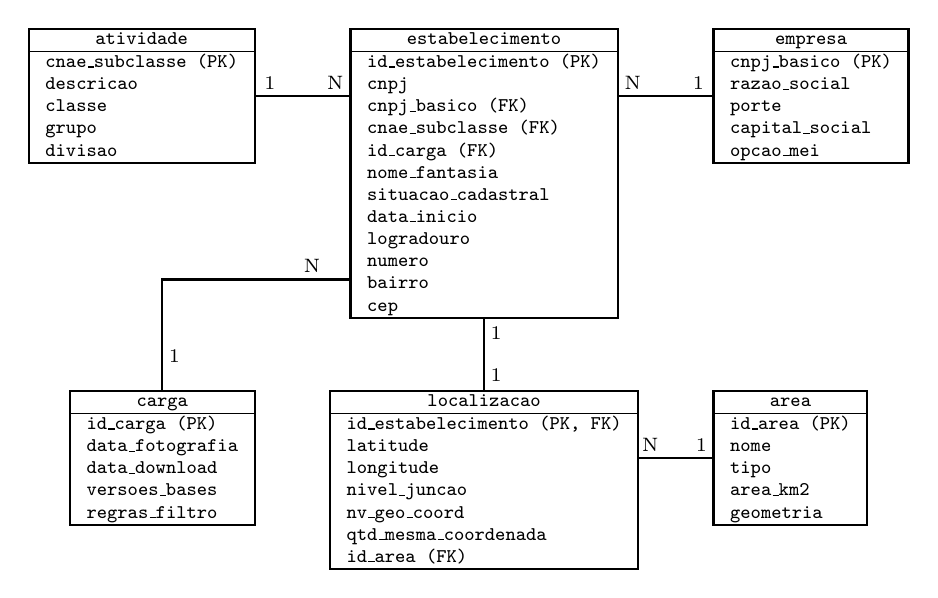
\begin{tikzpicture}[
        tabela/.style={
            draw=black,
            thick,
            inner sep=0pt,
            font=\scriptsize\ttfamily,
            fill=white
        },
        rel/.style={thick},
        card/.style={font=\scriptsize, inner sep=2pt}
    ]
        \node[tabela, anchor=north] (estab) at (0,0) {%
            \begin{tabular}{l}
                \multicolumn{1}{c}{\textbf{estabelecimento}} \\ \hline
                id\_estabelecimento (PK) \\
                cnpj \\
                cnpj\_basico (FK) \\
                cnae\_subclasse (FK) \\
                id\_carga (FK) \\
                nome\_fantasia \\
                situacao\_cadastral \\
                data\_inicio \\
                logradouro \\
                numero \\
                bairro \\
                cep
            \end{tabular}};

        \node[tabela, anchor=north east] (ativ) at (-2.9,0) {%
            \begin{tabular}{l}
                \multicolumn{1}{c}{\textbf{atividade}} \\ \hline
                cnae\_subclasse (PK) \\
                descricao \\
                classe \\
                grupo \\
                divisao
            \end{tabular}};

        \node[tabela, anchor=north west] (empresa) at (2.9,0) {%
            \begin{tabular}{l}
                \multicolumn{1}{c}{\textbf{empresa}} \\ \hline
                cnpj\_basico (PK) \\
                razao\_social \\
                porte \\
                capital\_social \\
                opcao\_mei
            \end{tabular}};

        \node[tabela, below=0.9cm of estab] (loc) {%
            \begin{tabular}{l}
                \multicolumn{1}{c}{\textbf{localizacao}} \\ \hline
                id\_estabelecimento (PK, FK) \\
                latitude \\
                longitude \\
                nivel\_juncao \\
                nv\_geo\_coord \\
                qtd\_mesma\_coordenada \\
                id\_area (FK)
            \end{tabular}};

        \node[tabela, anchor=north east] (carga) at (ativ.east |- loc.north) {%
            \begin{tabular}{l}
                \multicolumn{1}{c}{\textbf{carga}} \\ \hline
                id\_carga (PK) \\
                data\_fotografia \\
                data\_download \\
                versoes\_bases \\
                regras\_filtro
            \end{tabular}};

        \node[tabela, anchor=north west] (area) at (empresa.west |- loc.north) {%
            \begin{tabular}{l}
                \multicolumn{1}{c}{\textbf{area}} \\ \hline
                id\_area (PK) \\
                nome \\
                tipo \\
                area\_km2 \\
                geometria
            \end{tabular}};

        \draw[rel] (ativ.east) -- node[card, pos=0.15, above] {1} node[card, pos=0.85, above] {N} (ativ.east -| estab.west);
        \draw[rel] (empresa.west) -- node[card, pos=0.15, above] {1} node[card, pos=0.85, above] {N} (empresa.west -| estab.east);
        \draw[rel] (estab.south) -- node[card, pos=0.2, right] {1} node[card, pos=0.8, right] {1} (loc.north);
        \draw[rel] (carga.north) |- node[card, pos=0.15, right] {1} node[card, pos=0.9, above] {N} ([yshift=0.5cm]estab.south west);
        \draw[rel] (area.west) -- node[card, pos=0.15, above] {1} node[card, pos=0.85, above] {N} (area.west -| loc.east);
    \end{tikzpicture}
    \vspace{-0.2cm}
    \\\textbf{\footnotesize Fonte: Elaborado pelo autor.}
\end{figure}


Na terceira etapa ocorreu a implementação da solução.
Foi desenvolvida uma aplicação web na arquitetura cliente/servidor, organizada em três partes: o programa de carga, o banco de dados e a aplicação que o visitante usa no navegador.
O programa de carga importa e trata os arquivos; o banco guarda o resultado da fotografia; a aplicação consulta esse banco e entrega mapa, indicadores e tabela já filtrados.

As tecnologias utilizadas foram Python no programa de carga, MySQL no armazenamento, SvelteKit na aplicação web e Leaflet com \textit{tiles} do OpenStreetMap no mapa.
O sistema opera com dados estáticos: a base reflete o momento em que os arquivos foram carregados, e não é atualizada em tempo real a cada acesso.
Quando as fontes oficiais mudam, os dados da aplicação ficam desatualizados até que seja feita uma nova carga, com outra data de fotografia.

Na quarta etapa ocorreram os testes.
Foi aplicada a System Usability Scale (SUS) após os participantes usarem a interface, conforme descrito na Seção \ref{subsec:testes}.
Também foi conferida, de forma aproximada, a localização de uma amostra de endereços em outra fonte, sem substituir o CNEFE na base inteira.
Os totais da base foram comparados com os do CEMPRE, observando a ordem de grandeza e não a igualdade estrita dos números.

\section{O Software Desenvolvido}

Esta seção apresenta a aplicação construída a partir do projeto descrito na metodologia.
A tela principal reúne, sobre a mesma base de dados, os indicadores gerais do setor, a distribuição por subclasse e por porte, o mapa de pontos dos estabelecimentos e a tabela com busca por nome.
Os filtros aplicados em qualquer parte atualizam as demais, de modo que indicadores, mapa e tabela descrevem o mesmo conjunto de estabelecimentos.
A data da fotografia das bases e a indicação de coordenada ficam visíveis na própria interface.

% Continuar daqui: descrever as telas com capturas e a carga dos dados.

\subsection{Testes e análise}
\label{subsec:testes}

Foram realizados testes de usabilidade no sistema por meio do método System Usability Scale (SUS) \cite{brooke1996}.
Cinco participantes percorreram a aplicação com um roteiro curto: consultar os indicadores gerais, aplicar filtros por subclasse e por porte, localizar estabelecimentos no mapa e buscar um registro na tabela.
Em seguida, cada um respondeu aos dez itens do SUS, em escala Likert de 1 (discordo totalmente) a 5 (concordo totalmente), sem discussão prévia entre os respondentes.

A pontuação de cada participante foi calculada conforme \citeonline{brooke1996}: nos itens ímpares, subtraiu-se 1 da resposta; nos itens pares, subtraiu-se a resposta de 5; a soma dos dez valores foi multiplicada por 2,5, gerando um escore de 0 a 100.
A média dos cinco escores individuais foi 74,5.
Esse resultado situa-se acima da média de referência de 68 frequentemente citada para o SUS e, na escala de adjetivos de \citeonline{bangor2009}, aproxima-se da faixa associada a ``bom''.
A pontuação resume a percepção global de usabilidade e não identifica, sozinha, falhas pontuais de tela; eventuais comentários abertos dos participantes foram anotados apenas como apoio qualitativo à leitura do escore.

Além do SUS, uma amostra de cerca de 30 endereços foi conferida manualmente em mapa, para estimar, de forma aproximada, o afastamento entre o ponto atribuído e o endereço informado.
Essa conferência não substitui o CNEFE na base inteira.
Os detalhes numéricos da amostra e a comparação dos totais com o CEMPRE complementam a análise descritiva dos dados carregados.

\section{Considerações Finais}

Este trabalho partiu da dificuldade de consultar, de forma simples, dados abertos sobre as empresas de Tecnologia da Informação no município de Contagem.
As bases públicas existem, mas ficam dispersas e pouco acessíveis quando abertas só como arquivo bruto.
O objetivo geral foi desenvolver uma aplicação web interativa que caracterizasse e apresentasse esses estabelecimentos a partir da integração dessas fontes.

O primeiro objetivo específico --- coletar e tratar os dados, reunindo atividade, porte e localização --- foi alcançado com o programa em Python e a carga no MySQL, no recorte da divisão 62 em Contagem.
O segundo --- projetar a aplicação --- foi cumprido com o levantamento de requisitos, o diagrama de casos de uso e o esquema do banco.
O terceiro --- implementar a solução --- resultou na aplicação em SvelteKit, com mapa, indicadores, tabela e filtros sobre a mesma base.
O quarto --- testar a aplicação --- foi atendido com a System Usability Scale e com a conferência aproximada de uma amostra de endereços; a média SUS de 74,5 indica usabilidade percebida na faixa associada a ``bom'', e a amostra de localização permanece estimativa, sem substituir o CNEFE na base inteira.

Assim, a resposta à questão de pesquisa é afirmativa: é possível combinar os dados disponibilizados pela legislação em um sistema interativo que facilite a consulta às empresas de TI de Contagem, com as limitações da fotografia das bases e da junção por endereço.

A contribuição técnica e prática está na aplicação aberta, sem cadastro, que reúne indicadores, mapa e tabela sobre o mesmo conjunto filtrado de estabelecimentos.
A contribuição acadêmica está em mostrar, em um recorte municipal concreto, como dados abertos nacionais podem ser integrados e avaliados quanto à usabilidade da interface em um trabalho de Sistemas de Informação.

Entre as dificuldades, destacam-se a junção do endereço do CNPJ com o CNEFE, que nem sempre encontra coordenada precisa, e o fato de a base refletir apenas o momento da carga.
Também ficou claro que atualizar os dados exige nova execução do pipeline, e não uma consulta automática às fontes a cada acesso.

Como proposta para trabalho futuro, a aplicação pode deixar de operar apenas com dados estáticos e passar a atualizar a base em tempo real, ou em ciclos automáticos próximos a isso.
Hoje a consulta depende de uma fotografia carregada manualmente; uma evolução natural é agendar novas cargas a partir das fontes oficiais, para que mapa, indicadores e tabela acompanhem as mudanças do cadastro sem nova intervenção a cada publicação.

%%%%%%%%%%%%%%%%%%%%%%%%%%%%%%%%%%%
%% FIM DO TEXTO
%%%%%%%%%%%%%%%%%%%%%%%%%%%%%%%%%%%

% \selectlanguage{brazil}
%%%%%%%%%%%%%%%%%%%%%%%%%%%%%%%%%%%
%% Inicio bibliografia
%%%%%%%%%%%%%%%%%%%%%%%%%%%%%%%%%%%

 \newpage
\singlespace{
\renewcommand\refname{REFERÊNCIAS}
\bibliography{bibliografia}
}

%Inclusão do arquivo abntex2-alf.bst como solução para adequação à ABNT NBR 10520:2023 quanto às citações, que não são mais em caixa-alta
\bibliographystyle{abntex2-alf}

\newpage
\singlespace
\section*{APÊNDICE A -- Questionário System Usability Scale (SUS)}

Instrumento aplicado aos participantes após o roteiro de tarefas, com a escala Likert de cinco pontos: 1 = discordo totalmente; 5 = concordo totalmente.

\begin{table}[htbp]
    \centering
    \caption{Questionário SUS aplicado}
    \label{tab:questionario-sus}
    \small
    \begin{tabular}{p{0.8cm}p{8.8cm}ccccc}
        \hline
        \textbf{Nº} & \textbf{Afirmação} & \textbf{1} & \textbf{2} & \textbf{3} & \textbf{4} & \textbf{5} \\
        \hline
        1  & Eu acho que gostaria de usar este sistema com frequência. & $\square$ & $\square$ & $\square$ & $\square$ & $\square$ \\
        2  & Achei o sistema desnecessariamente complexo. & $\square$ & $\square$ & $\square$ & $\square$ & $\square$ \\
        3  & Achei o sistema fácil de usar. & $\square$ & $\square$ & $\square$ & $\square$ & $\square$ \\
        4  & Acho que precisaria de ajuda de um técnico para conseguir usar este sistema. & $\square$ & $\square$ & $\square$ & $\square$ & $\square$ \\
        5  & Achei que as várias funções do sistema estavam bem integradas. & $\square$ & $\square$ & $\square$ & $\square$ & $\square$ \\
        6  & Achei que o sistema apresenta muita inconsistência. & $\square$ & $\square$ & $\square$ & $\square$ & $\square$ \\
        7  & Imagino que a maioria das pessoas aprenderia a usar este sistema rapidamente. & $\square$ & $\square$ & $\square$ & $\square$ & $\square$ \\
        8  & Achei o sistema muito complicado de usar. & $\square$ & $\square$ & $\square$ & $\square$ & $\square$ \\
        9  & Senti-me muito confiante usando o sistema. & $\square$ & $\square$ & $\square$ & $\square$ & $\square$ \\
        10 & Precisei aprender muitas coisas antes de conseguir usar o sistema. & $\square$ & $\square$ & $\square$ & $\square$ & $\square$ \\
        \hline
    \end{tabular}
    \par\vspace{3pt}\textbf{\footnotesize Fonte: Adaptado de \citeonline{brooke1996}.}
\end{table}


\end{document}
